\documentclass[11pt]{article}

\usepackage[letterpaper,margin=0.82in]{geometry}
\usepackage{graphicx}
\usepackage{booktabs}
\usepackage{tabularx}
\usepackage{amsmath,amssymb}
\usepackage{microtype}
\usepackage{setspace}
\usepackage{caption}
\usepackage{float}
\usepackage{xcolor}
\usepackage{hyperref}
\usepackage{fancyhdr}
\usepackage{titlesec}

\definecolor{navy}{HTML}{173B57}
\definecolor{linkblue}{HTML}{2C7FB8}
\hypersetup{
  colorlinks=true,
  linkcolor=navy,
  urlcolor=linkblue,
  citecolor=navy,
  pdftitle={Using OLS Regression to Predict Median House Values in Philadelphia},
  pdfauthor={Qiwen Bian, Manching Ho, Fujia Zheng}
}

\graphicspath{{./}}
\captionsetup{font=small,labelfont={bf,color=navy},justification=centering,skip=4pt}
\setstretch{1.04}
\setlength{\parindent}{0pt}
\setlength{\parskip}{0.35em}
\setlength{\tabcolsep}{5.5pt}
\setlength{\intextsep}{8pt plus 1pt minus 1pt}
\setlength{\textfloatsep}{10pt plus 2pt minus 2pt}
\renewcommand{\arraystretch}{1.10}

\titleformat{\section}{\Large\bfseries\color{navy}}{}{0pt}{}
\titleformat{\subsection}{\large\bfseries\color{navy}}{}{0pt}{}
\titlespacing*{\section}{0pt}{1.15em}{0.35em}
\titlespacing*{\subsection}{0pt}{0.85em}{0.25em}

\pagestyle{fancy}
\fancyhf{}
\fancyhead[L]{\small OLS Regression and Philadelphia House Values}
\fancyhead[R]{\small CPLN 671 / MUSA 500}
\fancyfoot[C]{\thepage}
\renewcommand{\headrulewidth}{0.35pt}

\newcommand{\var}[1]{\texttt{#1}}
\newcommand{\tabnote}[1]{\par\vspace{0.2em}{\footnotesize\textbf{Note.} #1}}

\title{\vspace{-1.1cm}\textbf{Using OLS Regression to Predict\\Median House Values in Philadelphia}}
\author{Qiwen Bian \and Manching Ho \and Fujia Zheng}
\date{CPLN 671 / MUSA 500}

\begin{document}
\maketitle
\thispagestyle{fancy}

\section{Introduction}

Median house value reflects both housing characteristics and neighborhood demand. This study examines how house values vary across Philadelphia's 2000 Census block groups with housing vacancy, detached single-family housing, educational attainment, and poverty.

The predictor choices follow the hedonic view that housing prices capitalize structural and neighborhood attributes (Rosen, 1974). Education and detached housing are expected to be positively associated with value, while vacancy and poverty are expected to be negatively associated. The analysis estimates conditional associations, not causal effects.

We begin by preparing the data and exploring its patterns, then estimate the regression model, check whether its assumptions hold, and finally compare its predictive performance against a simpler alternative.

\section{Methods}

\subsection{Data Cleaning and Exploratory Analysis}

The course-provided \var{RegressionData.csv} had already been cleaned from 1,816 to 1,720 block groups. The cleaning removed block groups with population below 40, no housing units, median house value below \$10,000, and one North Philadelphia observation with house value above \$800,000 but household income below \$8,000.

Before fitting anything, we looked at each variable's scale, spread, and shape through histograms, means, and standard deviations. Strongly right-skewed variables can pull a linear model around, so variables containing zero were transformed with $\log(1+x)$ and the rest with $\log(x)$. The regression therefore uses $\log(\mathrm{MEDHVAL})$ as the response, $\log(1+\mathrm{NBELPOV100})$ for poverty, and the original percentage variables for vacancy, detached housing, and education.

Next we checked how the predictors relate to each other. Large pairwise correlations would mean two predictors carry similar information, a problem known as multicollinearity, so we computed Pearson correlations among them. For variables $x$ and $y$,

\begin{equation}
r=\frac{\sum_{i=1}^{n}(x_i-\bar{x})(y_i-\bar{y})}
{\sqrt{\sum_{i=1}^{n}(x_i-\bar{x})^2}\sqrt{\sum_{i=1}^{n}(y_i-\bar{y})^2}}.
\end{equation}

Here, $r$ is the sample Pearson correlation coefficient; $x_i$ and $y_i$ are the observed values of variables $x$ and $y$ for block group $i$; $\bar{x}$ and $\bar{y}$ are their sample means; $i$ indexes the block groups; and $n=1{,}720$ is the sample size. The numerator sums the paired deviations of the two variables from their means, while the two square-root terms in the denominator scale that joint variation by the variation in each variable. Consequently, $r$ ranges from $-1$ to $1$: its sign indicates the direction of the linear association, its absolute magnitude indicates the strength of that association, and $r=0$ indicates no linear association. We left the response out of this table: multicollinearity is about predictors overlapping each other, whereas a strong predictor-response correlation is exactly what a good model wants.

\subsection{Multiple Regression Analysis}

Multiple regression relates one response to several predictors at once. That matters here because vacancy, housing type, education, and poverty may each relate to house value and also to each other; estimating them together isolates each predictor's partial association while holding the others fixed, and the four combine to give a fitted value for every block group.

The population model was

\begin{equation}
\begin{aligned}
\mathrm{LNMEDHVAL}={}&\beta_0+\beta_1\mathrm{PCTVACANT}+\beta_2\mathrm{PCTSINGLES}\\
&+\beta_3\mathrm{PCTBACHMOR}+\beta_4\mathrm{LNNBELPOV100}+\varepsilon.
\end{aligned}
\end{equation}

In this equation, $\mathrm{LNMEDHVAL}$ is the natural logarithm of median house value. $\mathrm{PCTVACANT}$ is the percentage of housing units that are vacant, $\mathrm{PCTSINGLES}$ is the percentage of units that are detached single-family homes, $\mathrm{PCTBACHMOR}$ is the percentage of residents with a bachelor's degree or higher, and $\mathrm{LNNBELPOV100}$ is $\log(1+\mathrm{NBELPOV100})$, the transformed count of households living in poverty. The intercept $\beta_0$ is the expected log house value when all four predictors equal zero. Each slope $\beta_j$, for $j=1,\ldots,4$, is the expected change in log house value associated with a one-unit increase in its predictor while the other predictors are held fixed. The error term $\varepsilon$ represents omitted influences and random variation not captured by the four predictors.

OLS estimation and inference are only as trustworthy as the assumptions behind them. \textbf{Linearity} means that the conditional mean of the response is a linear combination of the included predictors and coefficients. If the true relationships are curved or otherwise nonlinear, fitted values and coefficient interpretations can be systematically distorted.

\textbf{Independence of observations} means that, after conditioning on the predictors, one block group's error does not provide information about another block group's error. If nearby block groups have correlated errors, the coefficient estimates can still describe the fitted sample relationship, but conventional standard errors and significance tests may be too optimistic.

\textbf{Homoscedasticity}, or constant error variance, means that the spread of the errors is approximately the same across all fitted values and predictor levels. If the error variance changes systematically, OLS coefficients remain centered on the specified linear relationship under the other assumptions, but the usual standard errors, confidence intervals, and tests may be unreliable.

\textbf{Normality of residuals} means that the errors are approximately normally distributed around zero. Normality is especially important for exact small-sample t-tests and F-tests; strong skewness or heavy tails can make those inferential results less accurate and can signal influential observations.

\textbf{No perfect multicollinearity} means that no predictor is an exact linear combination of the others, so every coefficient can be estimated separately. Perfect multicollinearity makes $\mathbf{X}^{\mathsf T}\mathbf{X}$ noninvertible, while very strong but imperfect multicollinearity can inflate standard errors and make individual coefficients unstable.

Under these assumptions, the unknown parameters are $\beta_0,\ldots,\beta_4$ and $\sigma^2=\operatorname{Var}(\varepsilon)$. OLS estimates

\begin{equation}
\widehat{\boldsymbol{\beta}}=(\mathbf{X}^{\mathsf T}\mathbf{X})^{-1}\mathbf{X}^{\mathsf T}\mathbf{y},
\qquad
\widehat{\sigma}^2=\frac{\sum e_i^2}{n-k-1}.
\end{equation}

Here, $\widehat{\boldsymbol{\beta}}$ is the vector of estimated coefficients, including the intercept. $\mathbf{X}$ is the design matrix with $n=1{,}720$ rows and $k+1$ columns, where $k=4$ is the number of predictors and the first column consists of ones for the intercept. $\mathbf{X}^{\mathsf T}$ is the transpose of the design matrix, $(\mathbf{X}^{\mathsf T}\mathbf{X})^{-1}$ is the inverse of its cross-product matrix, and $\mathbf{y}$ is the $n$-element vector of observed log house values. The estimator finds the coefficient values that minimize the sum of squared residuals. In the variance expression, $e_i=y_i-\widehat{y}_i$ is the residual for block group $i$, $\sum e_i^2$ is the residual sum of squares, $n-k-1$ is the residual degrees of freedom, and $\widehat{\sigma}^2$ estimates the error variance $\sigma^2$.

To summarize fit once the coefficients were estimated, we used

\begin{equation}
R^2=1-\frac{SS_{\mathrm{res}}}{SS_{\mathrm{tot}}},
\qquad
\bar{R}^2=1-\frac{SS_{\mathrm{res}}/(n-k-1)}{SS_{\mathrm{tot}}/(n-1)}.
\end{equation}

In these expressions, $SS_{\mathrm{res}}=\sum_{i=1}^{n}(y_i-\widehat{y}_i)^2$ is the sum of squared residuals, which measures the variation left unexplained by the model. $SS_{\mathrm{tot}}=\sum_{i=1}^{n}(y_i-\bar{y})^2$ is the total sum of squares, which measures the total variation in the response around its sample mean $\bar{y}$. As above, $n=1{,}720$ is the number of observations and $k=4$ is the number of predictors. $R^2$ is the fraction of the response variation explained by the fitted model. Adjusted $R^2$, denoted $\bar{R}^2$, penalizes the addition of predictors by accounting for the model and residual degrees of freedom, so it increases only when an added predictor improves fit sufficiently.

Statistical tests complement these descriptive fit measures. The overall F-test evaluates $H_0:\beta_1=\cdots=\beta_4=0$, meaning that none of the four predictors has a linear association with log house value after the others are included, against the alternative that at least one slope is nonzero. Each two-sided t-test evaluates $H_0:\beta_j=0$, meaning that predictor $j$ has no conditional linear association with log house value, against $H_a:\beta_j\ne0$.

\subsection{Additional Analyses and Software}

We then ran two extra checks: model selection and out-of-sample prediction. Stepwise regression tries adding (forward selection) or removing (backward elimination) predictors one at a time, keeping changes that improve a stated criterion. It can suggest a simpler model, but the result depends on the sample and does not by itself validate the regression assumptions.

Backward and forward stepwise comparison used the \var{step} function and

\begin{equation}
\mathrm{AIC}=-2\log(L)+2k.
\end{equation}

In this equation, $\mathrm{AIC}$ is the Akaike information criterion, $L$ is the maximized likelihood of the fitted model, and $\log(L)$ is the log-likelihood, which measures how well the model fits the observed data. In the AIC equation only, $k$ denotes the number of estimated parameters, so the term $2k$ penalizes model complexity. Lower AIC indicates a better trade-off between fit and complexity among models fit to the same data. However, stepwise results remain sample-dependent and do not repair misspecification or spatial dependence.

Five-fold cross-validation then tested out-of-sample prediction: we divided the 1,720 block groups into five folds, trained on four while predicting the fifth, and rotated until every fold had served as the test set once, so each block group received a prediction from a model that had never seen it. The procedure compared the four-predictor model with a model containing \var{PCTVACANT} and \var{MEDHHINC}, using identical folds so the comparison would reflect model differences rather than different data partitions. Prediction error was

\begin{equation}
\mathrm{RMSE}=\sqrt{\frac{1}{n}\sum_{i=1}^{n}(y_i-\widehat{y}_{i,\mathrm{CV}})^2}.
\end{equation}

Here, $y_i$ is the observed log house value for block group $i$, and $\widehat{y}_{i,\mathrm{CV}}$ is its predicted value when block group $i$ belonged to the held-out fold. The index $i$ runs over all observations, and $n=1{,}720$ is the total number of block groups. Squaring prevents positive and negative errors from cancelling, averaging summarizes error over all observations, and the square root returns the measure to the response scale. RMSE therefore represents the typical prediction error in the same units as the response, with lower values indicating better predictive accuracy.

All analysis and graphics were done in R with \var{lm}, \var{step}, the fold-allocation algorithm used by \var{DAAG::CVlm}, and the \var{sf} and \var{classInt} spatial packages. The results below follow the same order: sample description and spatial patterns first, then regression estimates, assumption checks, and model comparisons.

\section{Results}

\subsection{Exploratory Results}

The cleaned sample contains 1,720 block groups, and Table~\ref{tab:summary} shows wide variation in house value and every predictor. That spread is what lets the regression distinguish the predictors' separate associations.

\begin{table}[H]
\centering
\caption{Summary statistics ($n=1{,}720$)}
\label{tab:summary}
\begin{tabular}{lrr}
\toprule
Variable & Mean & SD \\
\midrule
Median House Value (\$) & 66,287.73 & 60,006.08 \\
\% Bachelor's Degree or Higher & 16.08 & 17.77 \\
Households Living in Poverty & 189.77 & 164.32 \\
\% Vacant Housing Units & 11.29 & 9.63 \\
\% Detached Single-Family Units & 9.23 & 13.25 \\
\bottomrule
\end{tabular}
\end{table}

The original variables were right-skewed rather than normal. As Figure~\ref{fig:distributions} shows, logging made house value and poverty more symmetric; the other predictors kept their spikes at zero, so we kept their original forms. The remaining assumptions get checked below with bivariate plots and residual diagnostics.

\begin{figure}[p]
\centering
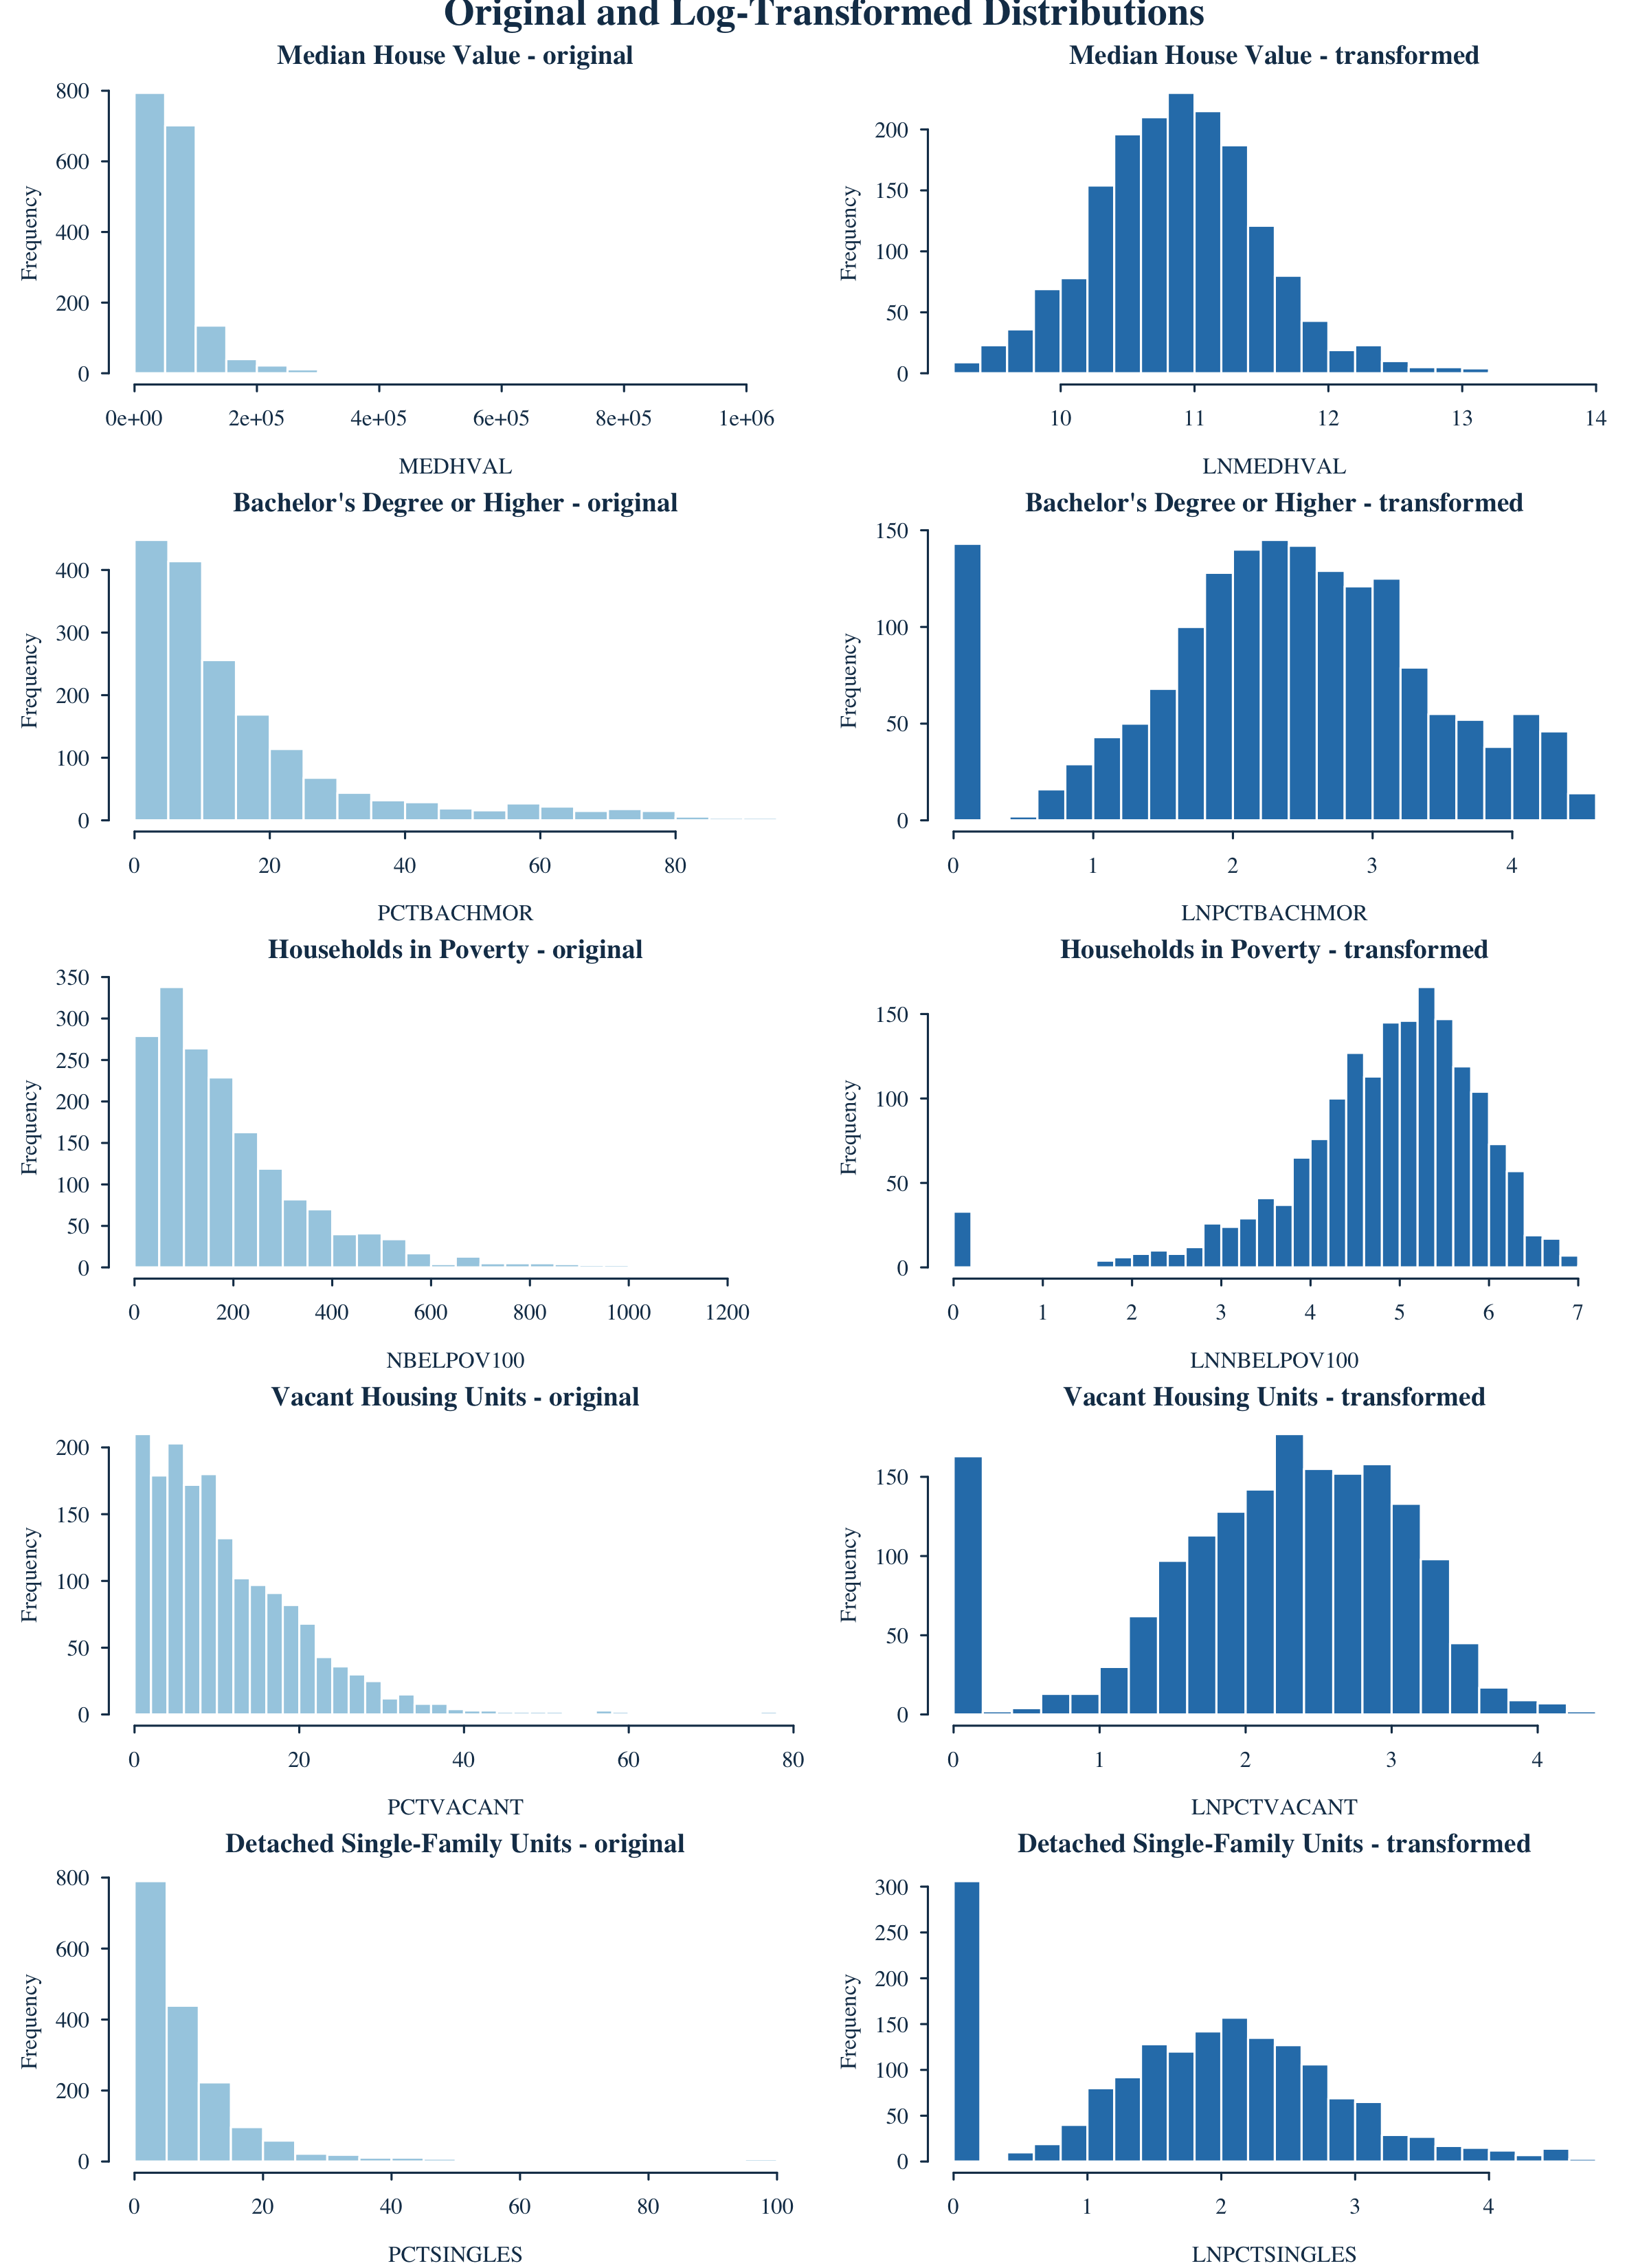
\includegraphics[width=0.72\textwidth,height=0.82\textheight,keepaspectratio]{fig_01_distributions.png}
\caption{Original and log-transformed variable distributions.}
\label{fig:distributions}
\end{figure}

Figures~\ref{fig:response-map} and~\ref{fig:predictor-maps} map the response and predictors on the same five-quantile blue-to-red scale, so the eye can compare them directly. House values are high in the Far Northeast, Northwest, and Center City and lower in much of North and West Philadelphia. Education broadly follows the house-value pattern, while vacancy and poverty often show the reverse. Detached housing is most similar to house value near the city's edges. The geographic clustering suggests spatial autocorrelation and possible dependence among nearby block groups, an issue revisited in the residual diagnostics.

\begin{figure}[p]
\centering
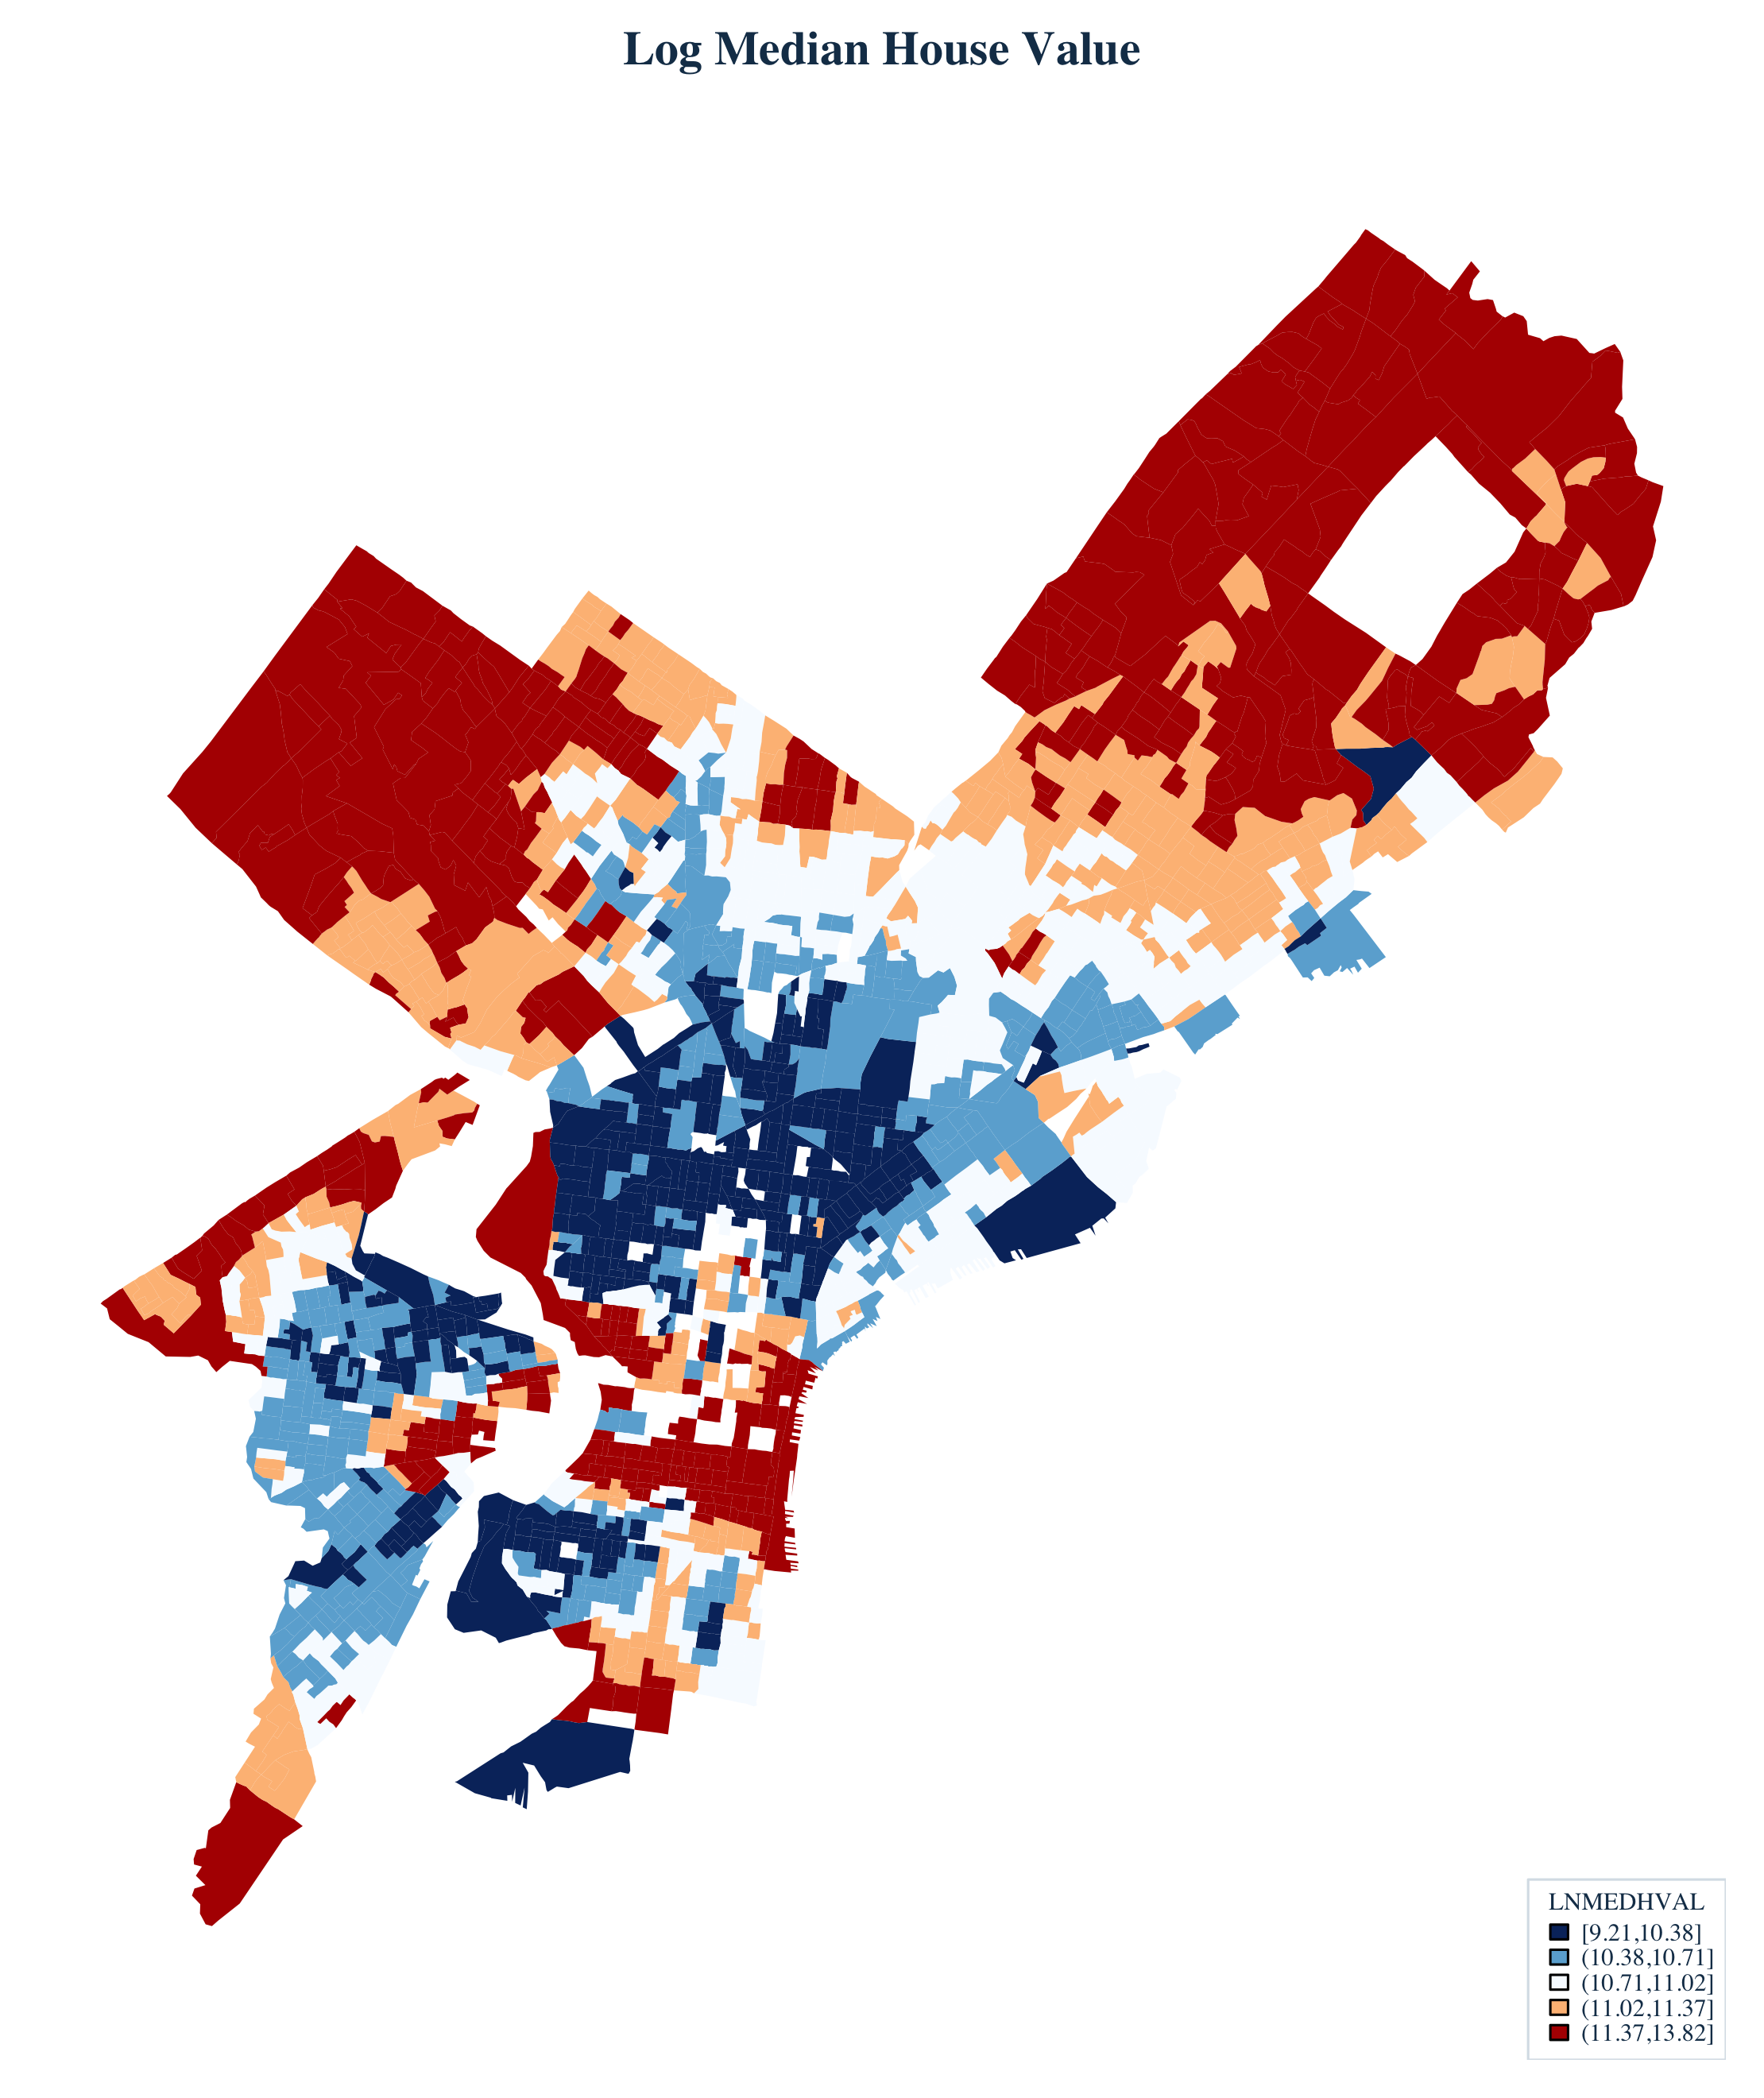
\includegraphics[width=0.67\textwidth,height=0.79\textheight,keepaspectratio]{fig_02_map_response.png}
\caption{Log median house value by block group.}
\label{fig:response-map}
\end{figure}

\begin{figure}[p]
\centering
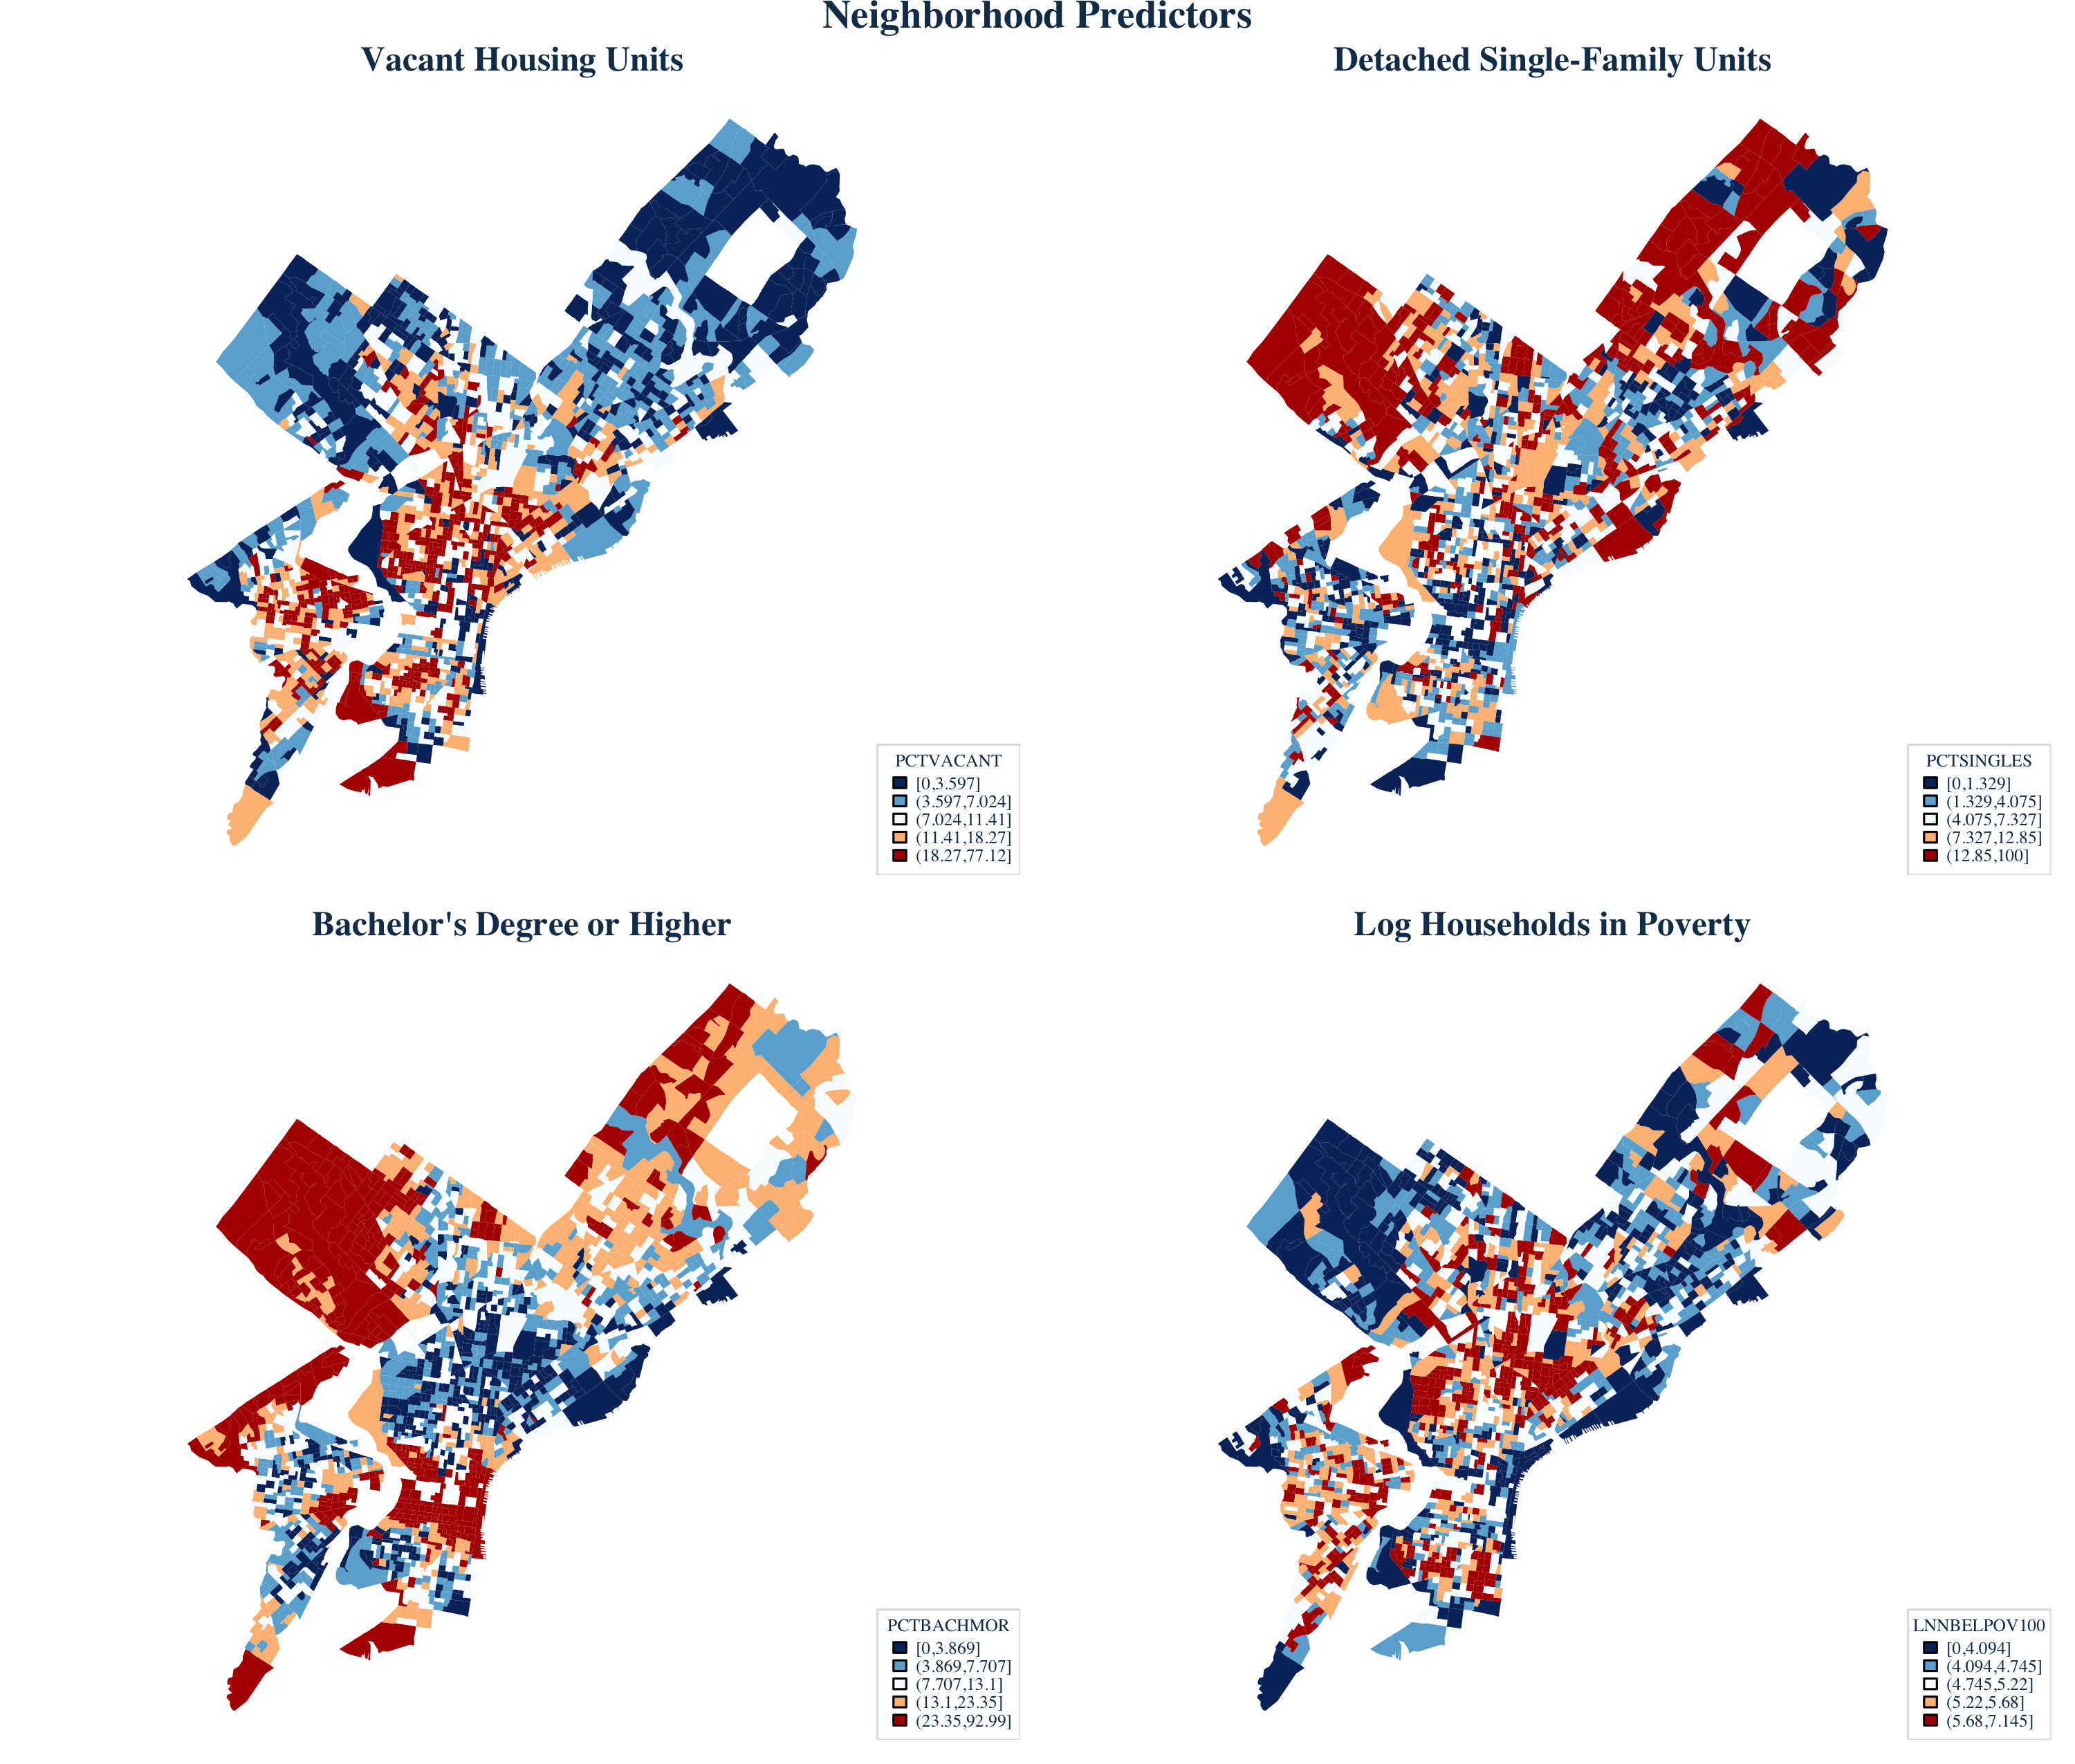
\includegraphics[width=0.95\textwidth,height=0.78\textheight,keepaspectratio]{fig_03_map_predictors.png}
\caption{Model predictors by block group.}
\label{fig:predictor-maps}
\end{figure}

Table~\ref{tab:correlations} puts numbers on those visual impressions: the largest absolute correlation is 0.320. The maps and correlations show related spatial patterns but no severe pairwise multicollinearity, so we can estimate all four predictors together and read off their partial associations.

\begin{table}[H]
\centering
\caption{Pearson correlations among predictors}
\label{tab:correlations}
\small
\begin{tabular}{lrrrr}
\toprule
 & \var{PCTVACANT} & \var{PCTSINGLES} & \var{PCTBACHMOR} & \var{LNNBELPOV100} \\
\midrule
\var{PCTVACANT} & 1.000 & & & \\
\var{PCTSINGLES} & $-0.151$ & 1.000 & & \\
\var{PCTBACHMOR} & $-0.298$ & 0.198 & 1.000 & \\
\var{LNNBELPOV100} & 0.250 & $-0.291$ & $-0.320$ & 1.000 \\
\bottomrule
\end{tabular}
\end{table}

\subsection{Regression Results}

The model was jointly significant, with every coefficient significant at $p<.001$ (Tables~\ref{tab:ols} and~\ref{tab:anova}). The F-test's null hypothesis is that all four slopes are zero once the predictors are considered together; with $F=840.857$ and $p<.001$, such an extreme result would be very unlikely under that null, giving strong evidence that at least one predictor is linearly related to log house value.

Vacancy's coefficient is $-0.0192$: holding the other predictors fixed, one more point of vacancy goes with roughly a 1.9\% lower median value, and its $p<.001$ rejects the null hypothesis of no conditional association. For detached housing (0.0030), a one-point rise goes with about a 0.3\% higher value, other things equal, again with $p<.001$. Education carries the largest percentage-point association (0.0209): one more point of bachelor's share goes with about a 2.1\% higher value, holding the rest fixed, with $p<.001$ firmly rejecting the null. Poverty enters on the log scale ($-0.0789$): a 10\% rise in the poverty count goes with about a 0.8\% lower value, conditional on the other predictors, and its $p<.001$ likewise rejects no association. All four signs match the expectations stated in the introduction, and $R^2=0.6623$ means the model accounts for 66.2\% of the variation in log house value.

\begin{table}[H]
\centering
\caption{OLS regression of \var{LNMEDHVAL}}
\label{tab:ols}
\begin{tabular}{lrrrr}
\toprule
Term & Coefficient & Std. Error & $t$ & $p$-value \\
\midrule
Intercept & 11.1138 & 0.0465 & 238.84 & $<.001$ \\
\var{PCTVACANT} & $-0.0192$ & 0.0010 & $-19.59$ & $<.001$ \\
\var{PCTSINGLES} & 0.0030 & 0.0007 & 4.23 & $<.001$ \\
\var{PCTBACHMOR} & 0.0209 & 0.0005 & 38.49 & $<.001$ \\
\var{LNNBELPOV100} & $-0.0789$ & 0.0085 & $-9.33$ & $<.001$ \\
\bottomrule
\end{tabular}
\tabnote{$R^2=0.6623$; adjusted $R^2=0.6615$; residual standard error $=0.3665$.}
\end{table}

\begin{table}[H]
\centering
\caption{Analysis of variance}
\label{tab:anova}
\begin{tabular}{lrrrrr}
\toprule
Source & df & Sum of Squares & Mean Square & $F$ & $p$-value \\
\midrule
Regression & 4 & 451.746 & 112.936 & 840.857 & $<.001$ \\
Error & 1,715 & 230.344 & 0.134 & & \\
Total & 1,719 & 682.089 & & & \\
\bottomrule
\end{tabular}
\end{table}

\subsection{Regression Assumption Checks}

Significant coefficients don't guarantee the assumptions hold, so we check them directly (distributions and multicollinearity were already covered). Figure~\ref{fig:scatterplots} plots each predictor against log house value and shows visible curvature, especially for vacancy and education. A straight line gets the general direction right, but it remains only an approximation.

\begin{figure}[p]
\centering
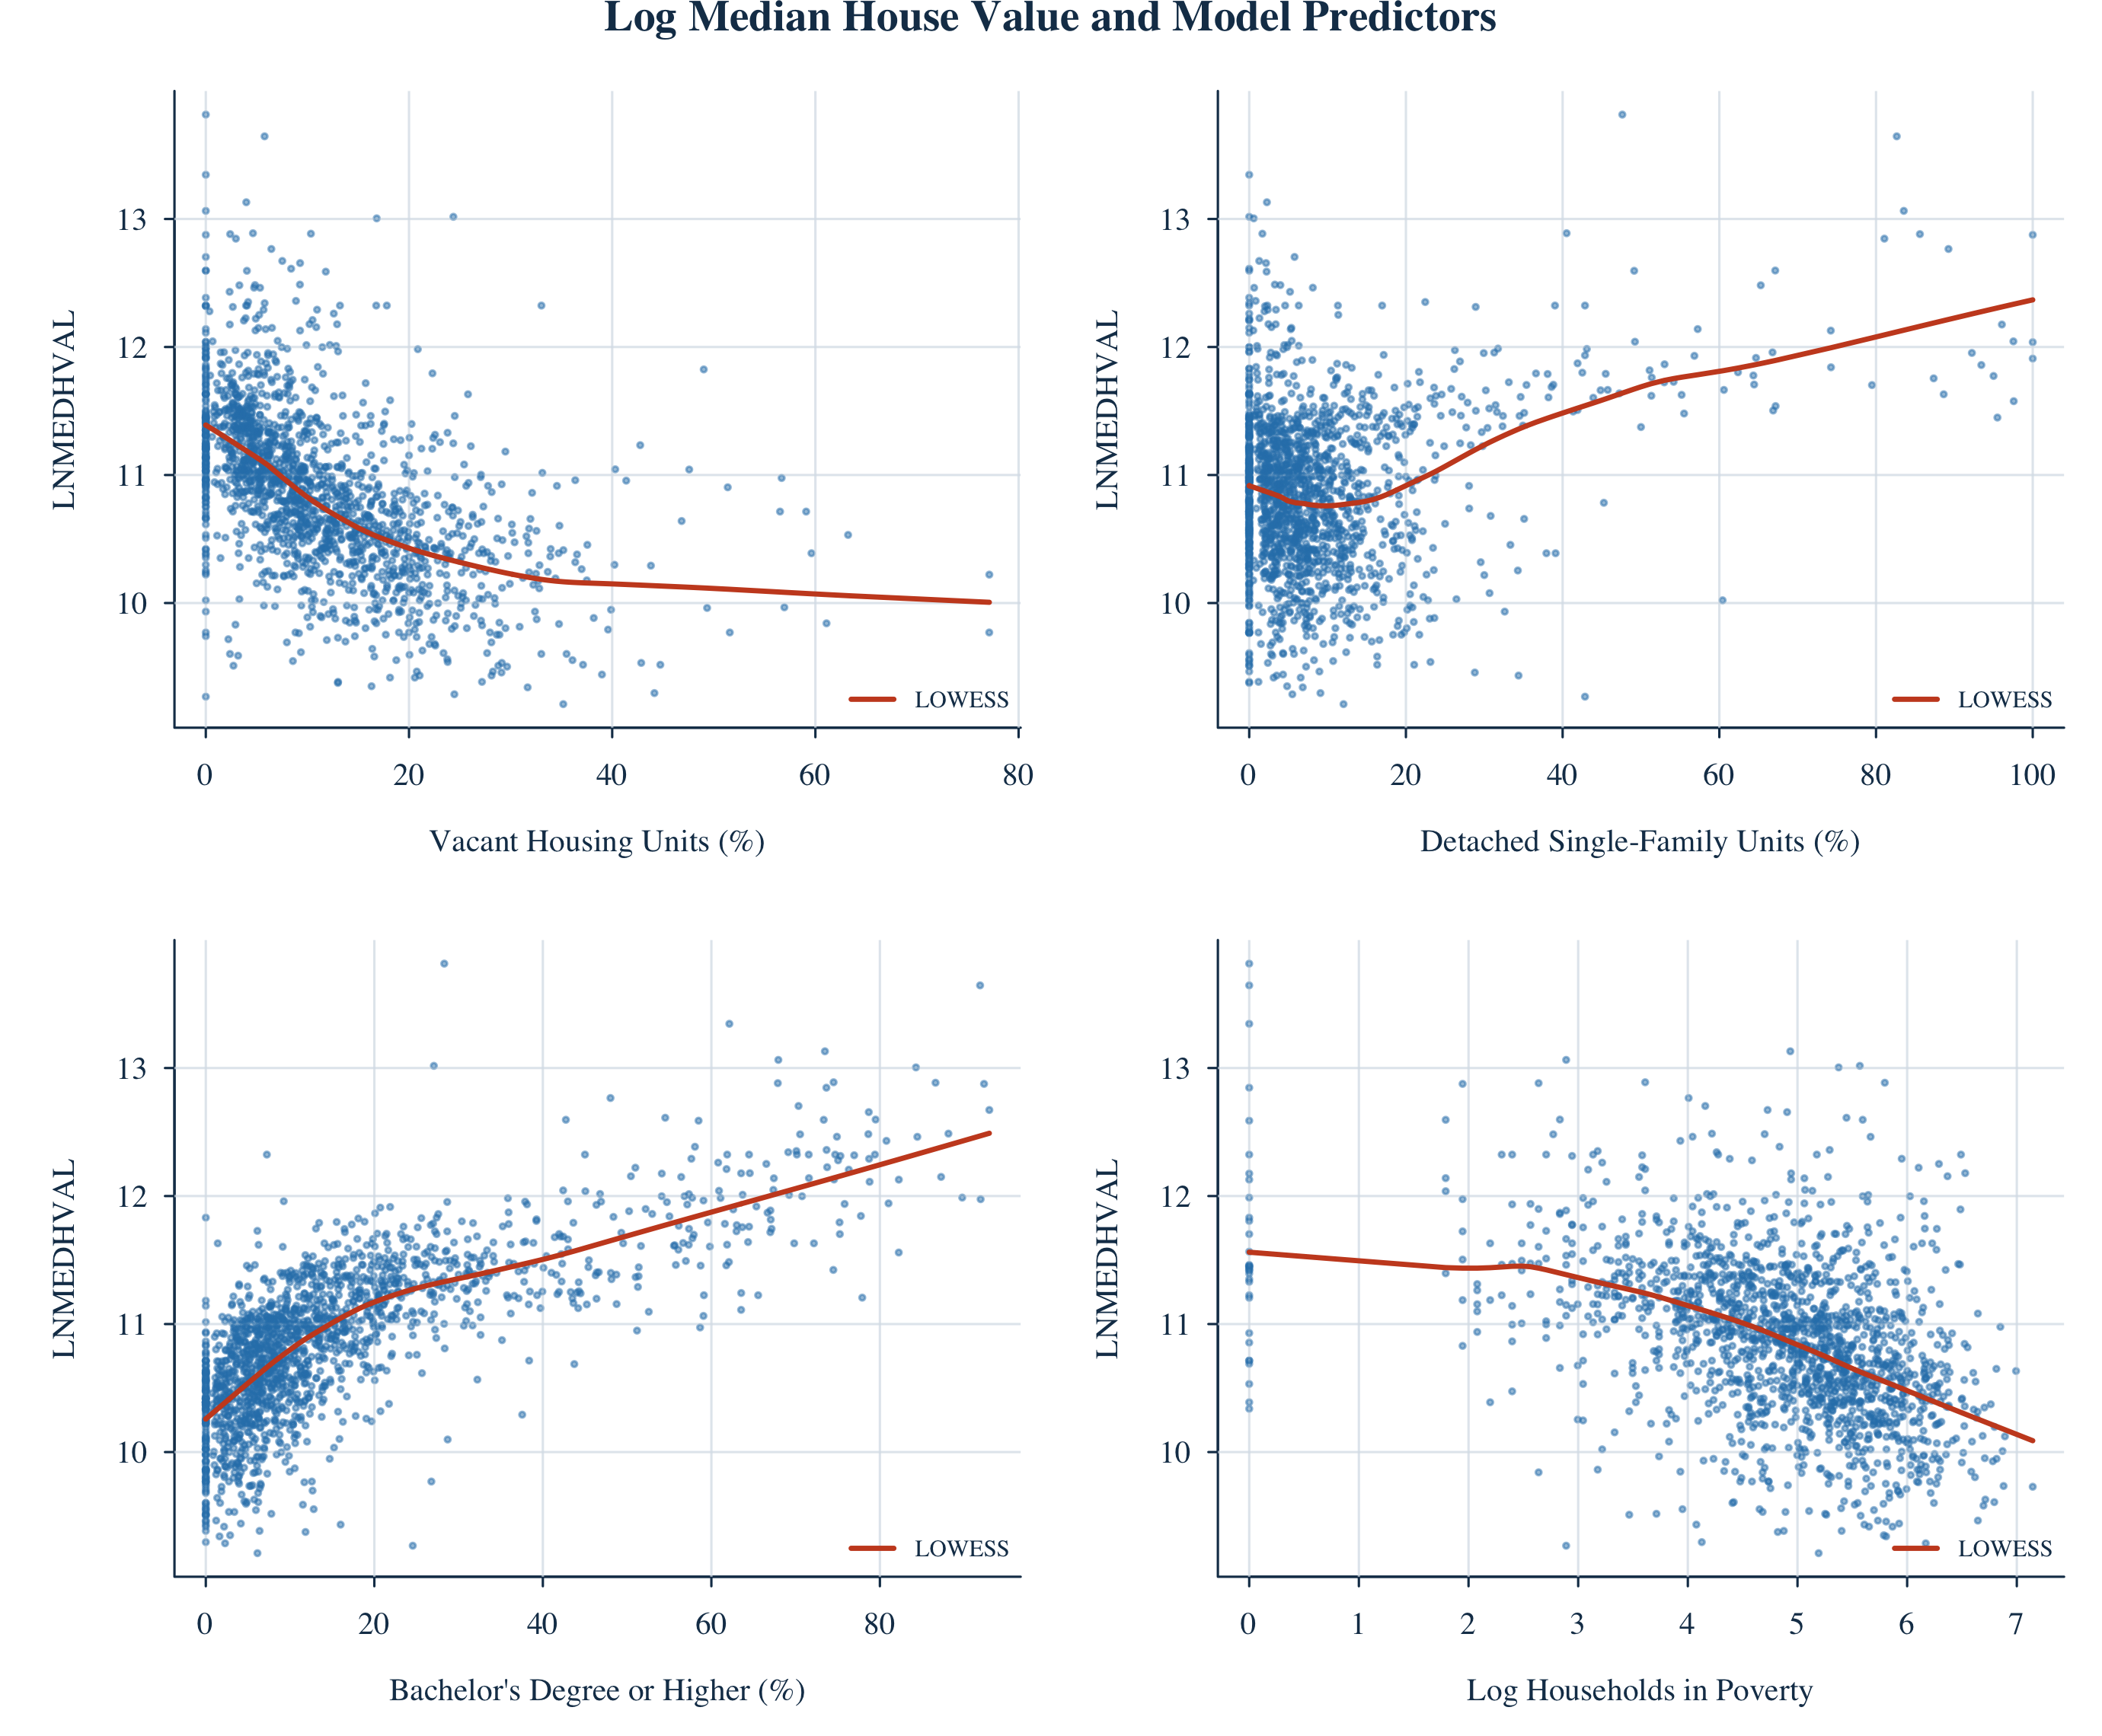
\includegraphics[width=0.94\textwidth,height=0.77\textheight,keepaspectratio]{fig_04_scatterplots.png}
\caption{Log median house value and model predictors, with LOWESS trends.}
\label{fig:scatterplots}
\end{figure}

Next, the errors themselves. A standardized residual is a raw residual divided by its estimated standard error, including a leverage adjustment, so observations can be compared on a common scale. Figure~\ref{fig:residual-histogram} is centered near zero but more sharply peaked and heavy-tailed than the normal reference; 20 observations have $|r_i|>3$. This departure from the reference shape weakens the normality assumption and suggests that exact small-sample inference should be interpreted cautiously. Figure~\ref{fig:residual-fitted} shows changing spread and several extreme errors, indicating mild heteroscedasticity; 85 observations, or 4.9\%, have $|r_i|>2$. The changing spread implies that the constant-variance assumption is not fully satisfied and may affect conventional standard errors.

\begin{figure}[p]
\centering
\begin{minipage}[t]{0.49\textwidth}
\centering
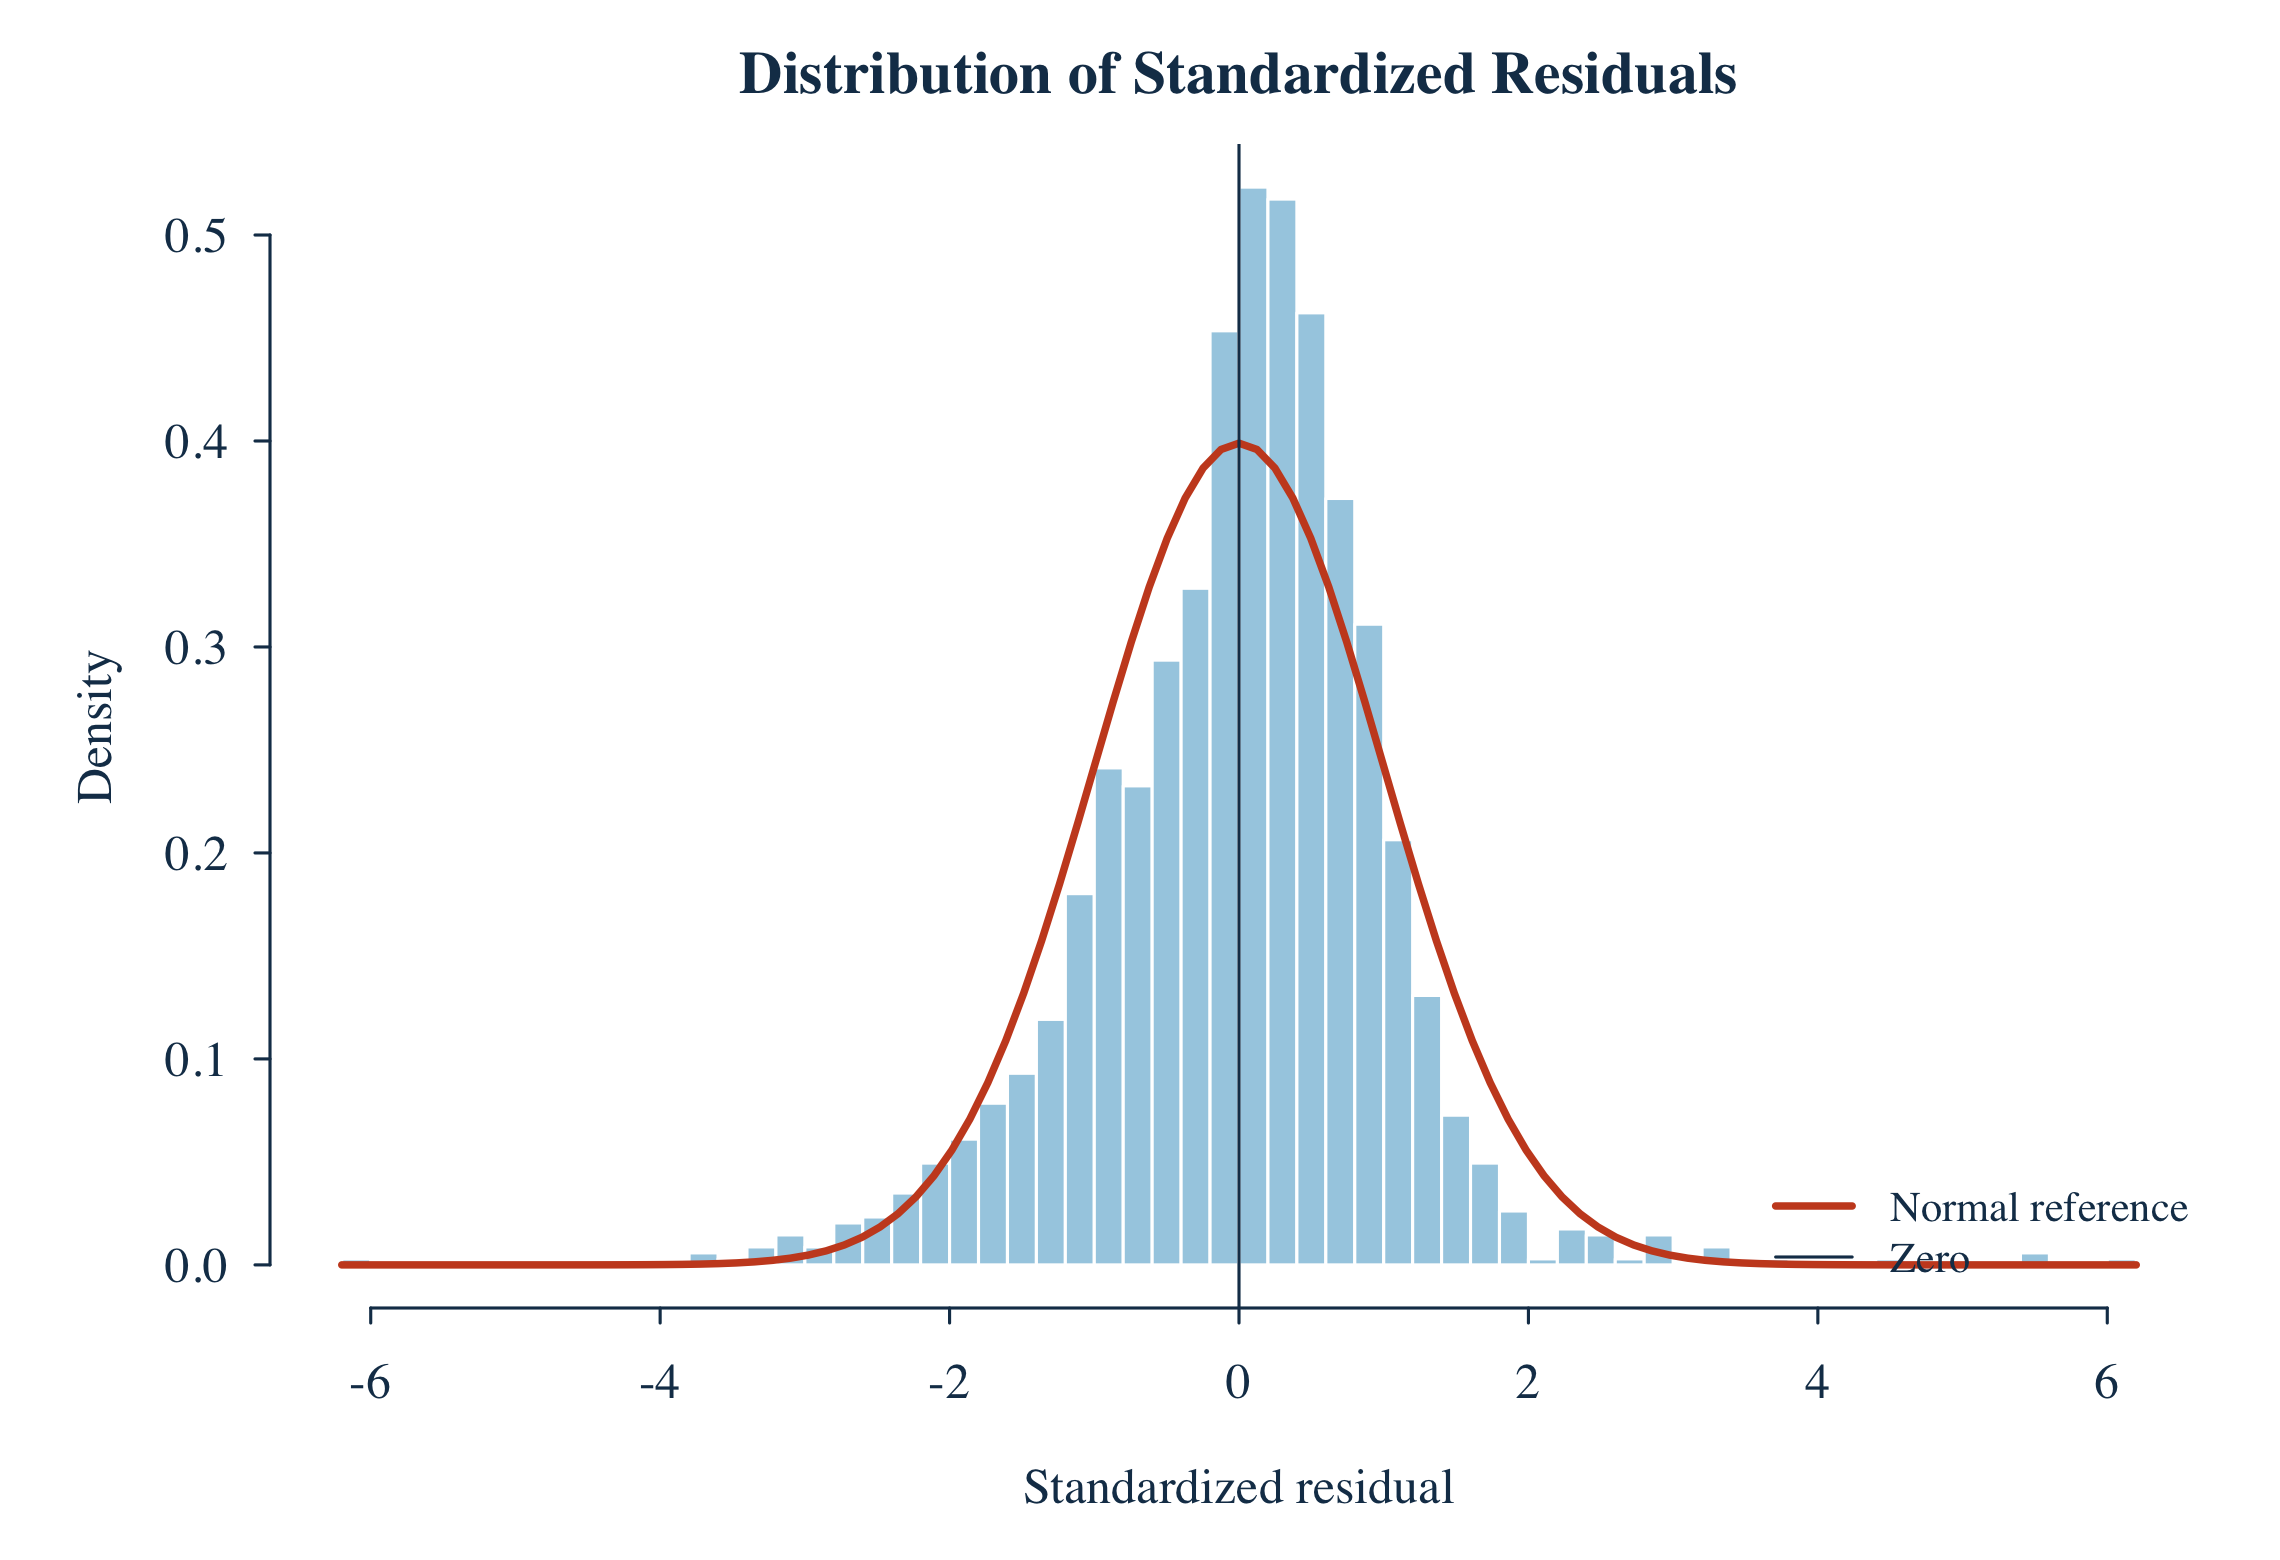
\includegraphics[width=\linewidth]{fig_05_residual_histogram.png}
\caption{Distribution of standardized residuals.}
\label{fig:residual-histogram}
\end{minipage}\hfill
\begin{minipage}[t]{0.49\textwidth}
\centering
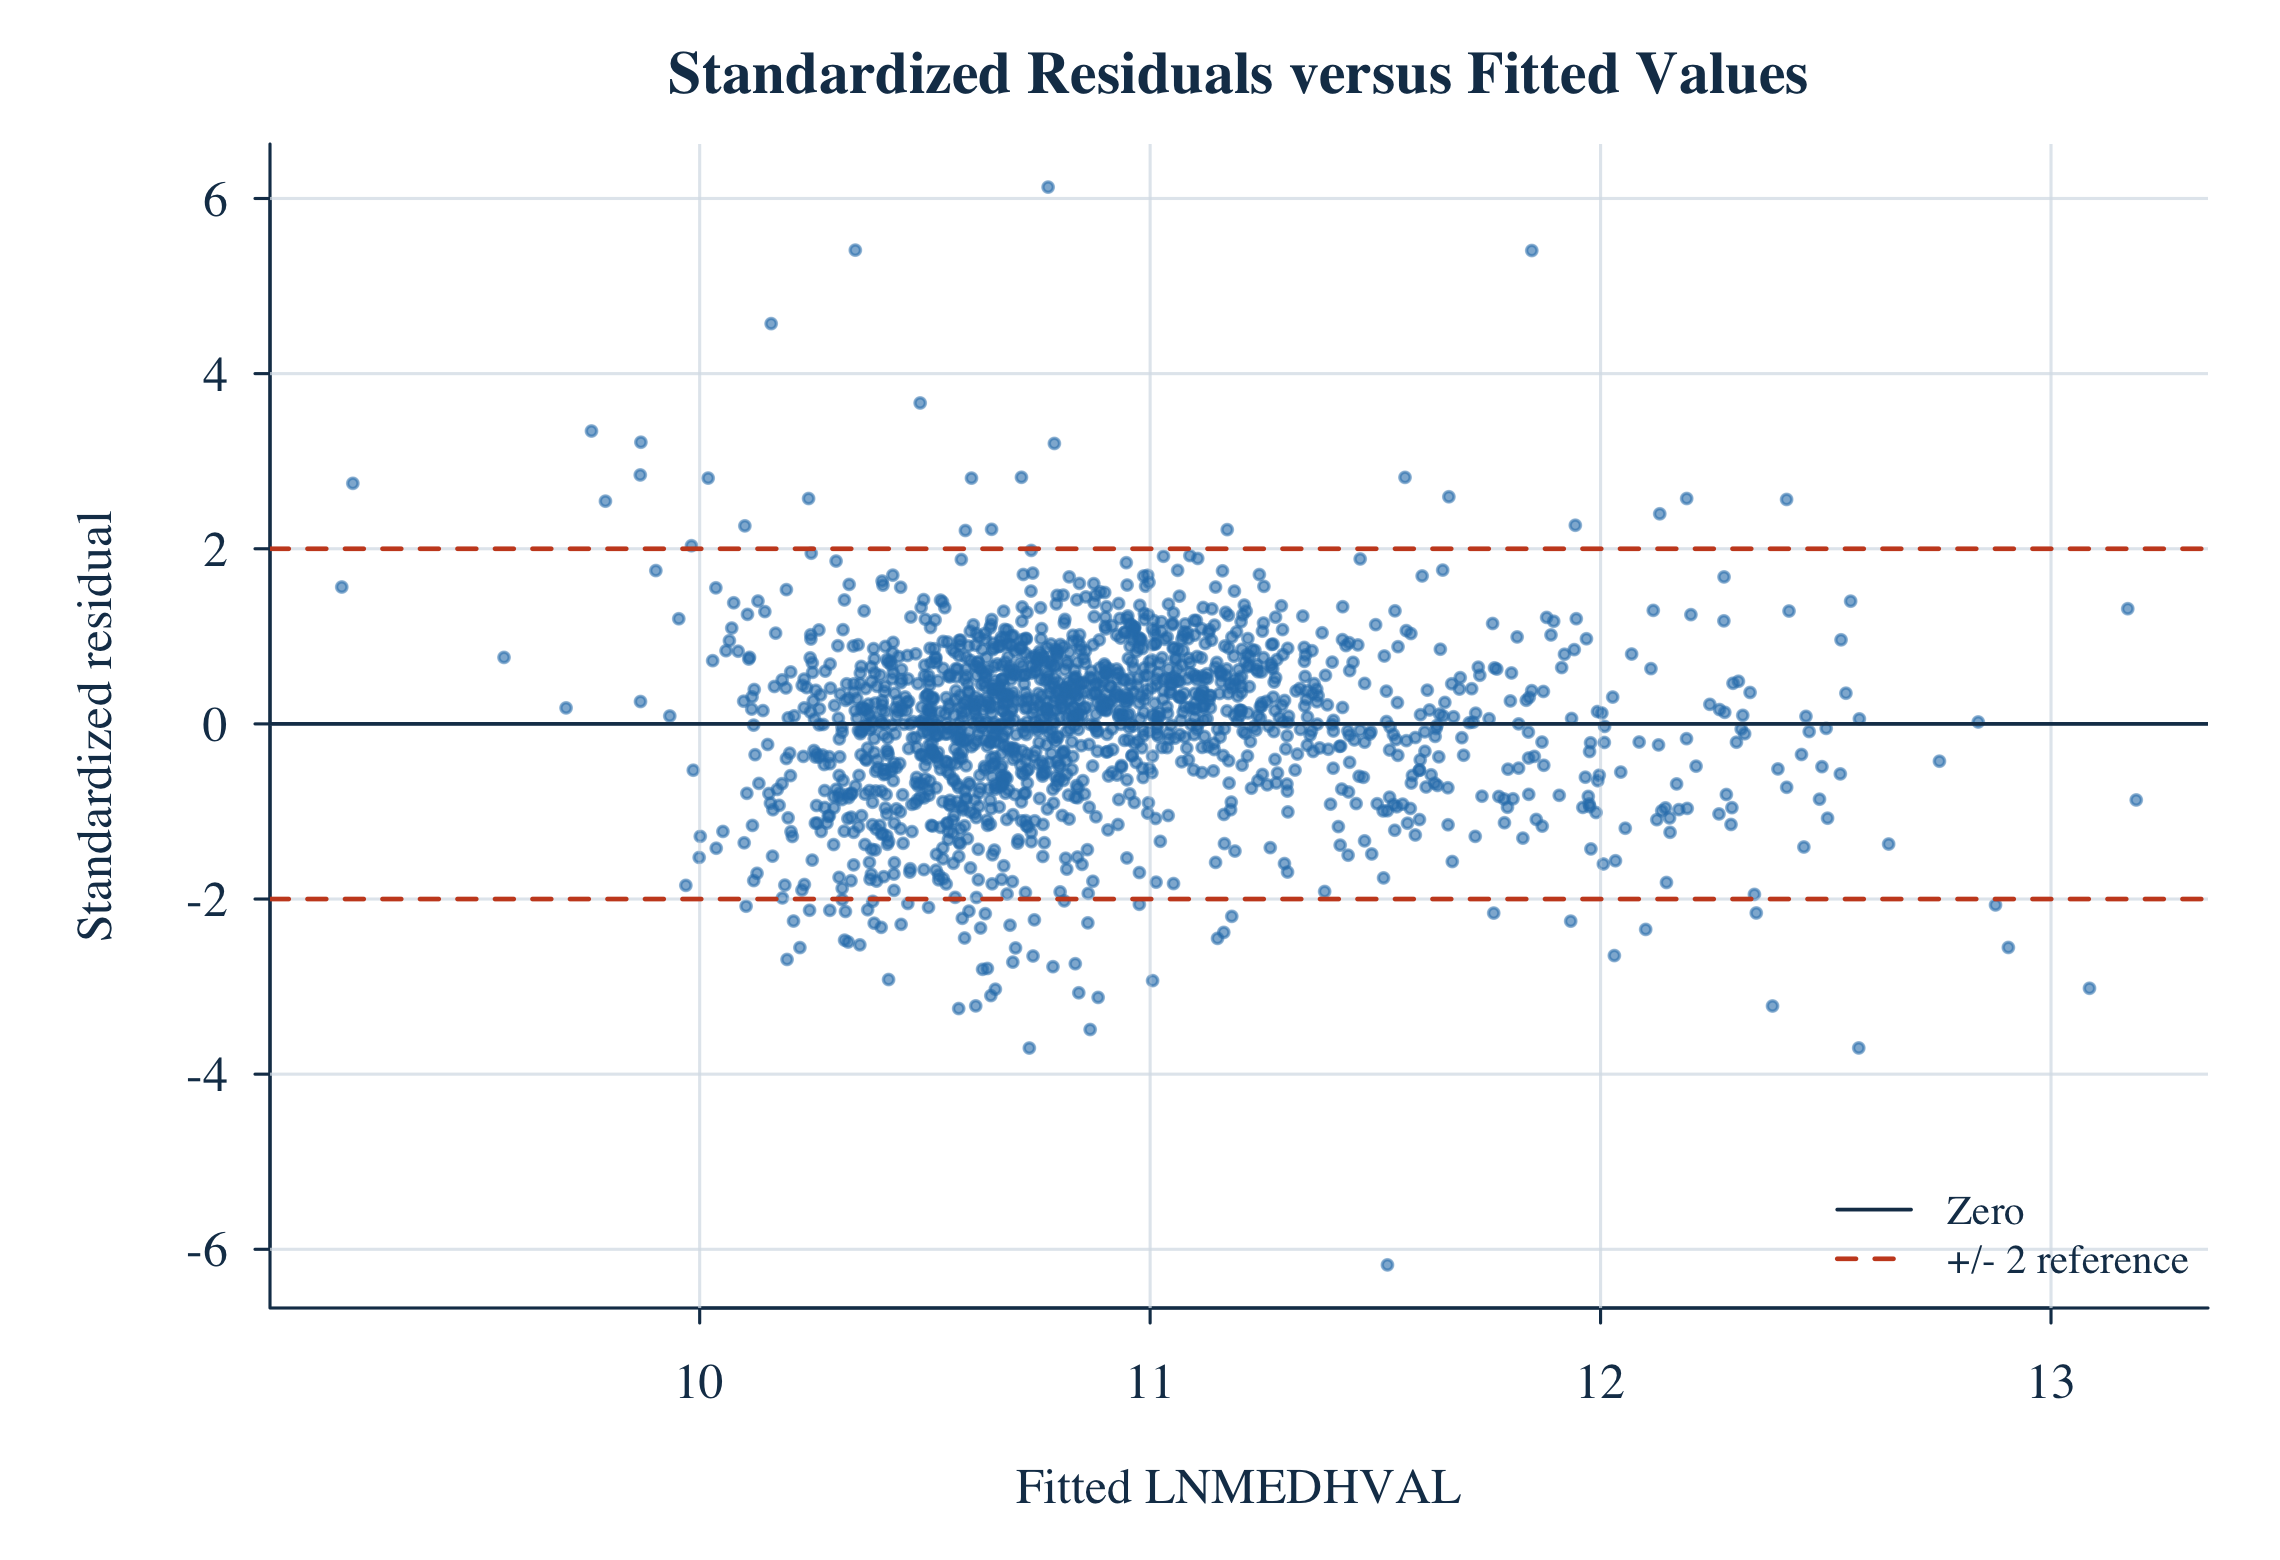
\includegraphics[width=\linewidth]{fig_06_residuals_vs_fitted.png}
\caption{Standardized residuals versus fitted values.}
\label{fig:residual-fitted}
\end{minipage}
\end{figure}

Finally, Figure~\ref{fig:residual-map} maps the residuals: instead of random scatter, we see regional clusters of positive and negative errors. This suggests spatially correlated residuals and a violation of independence, although a formal statistic such as Moran's I is needed for confirmation. Because the diagnostics reveal limitations in linearity, normality, constant variance, and independence, the model-comparison results that follow should be viewed as comparisons within the existing candidate set rather than proof that the OLS specification is fully adequate.

\begin{figure}[p]
\centering
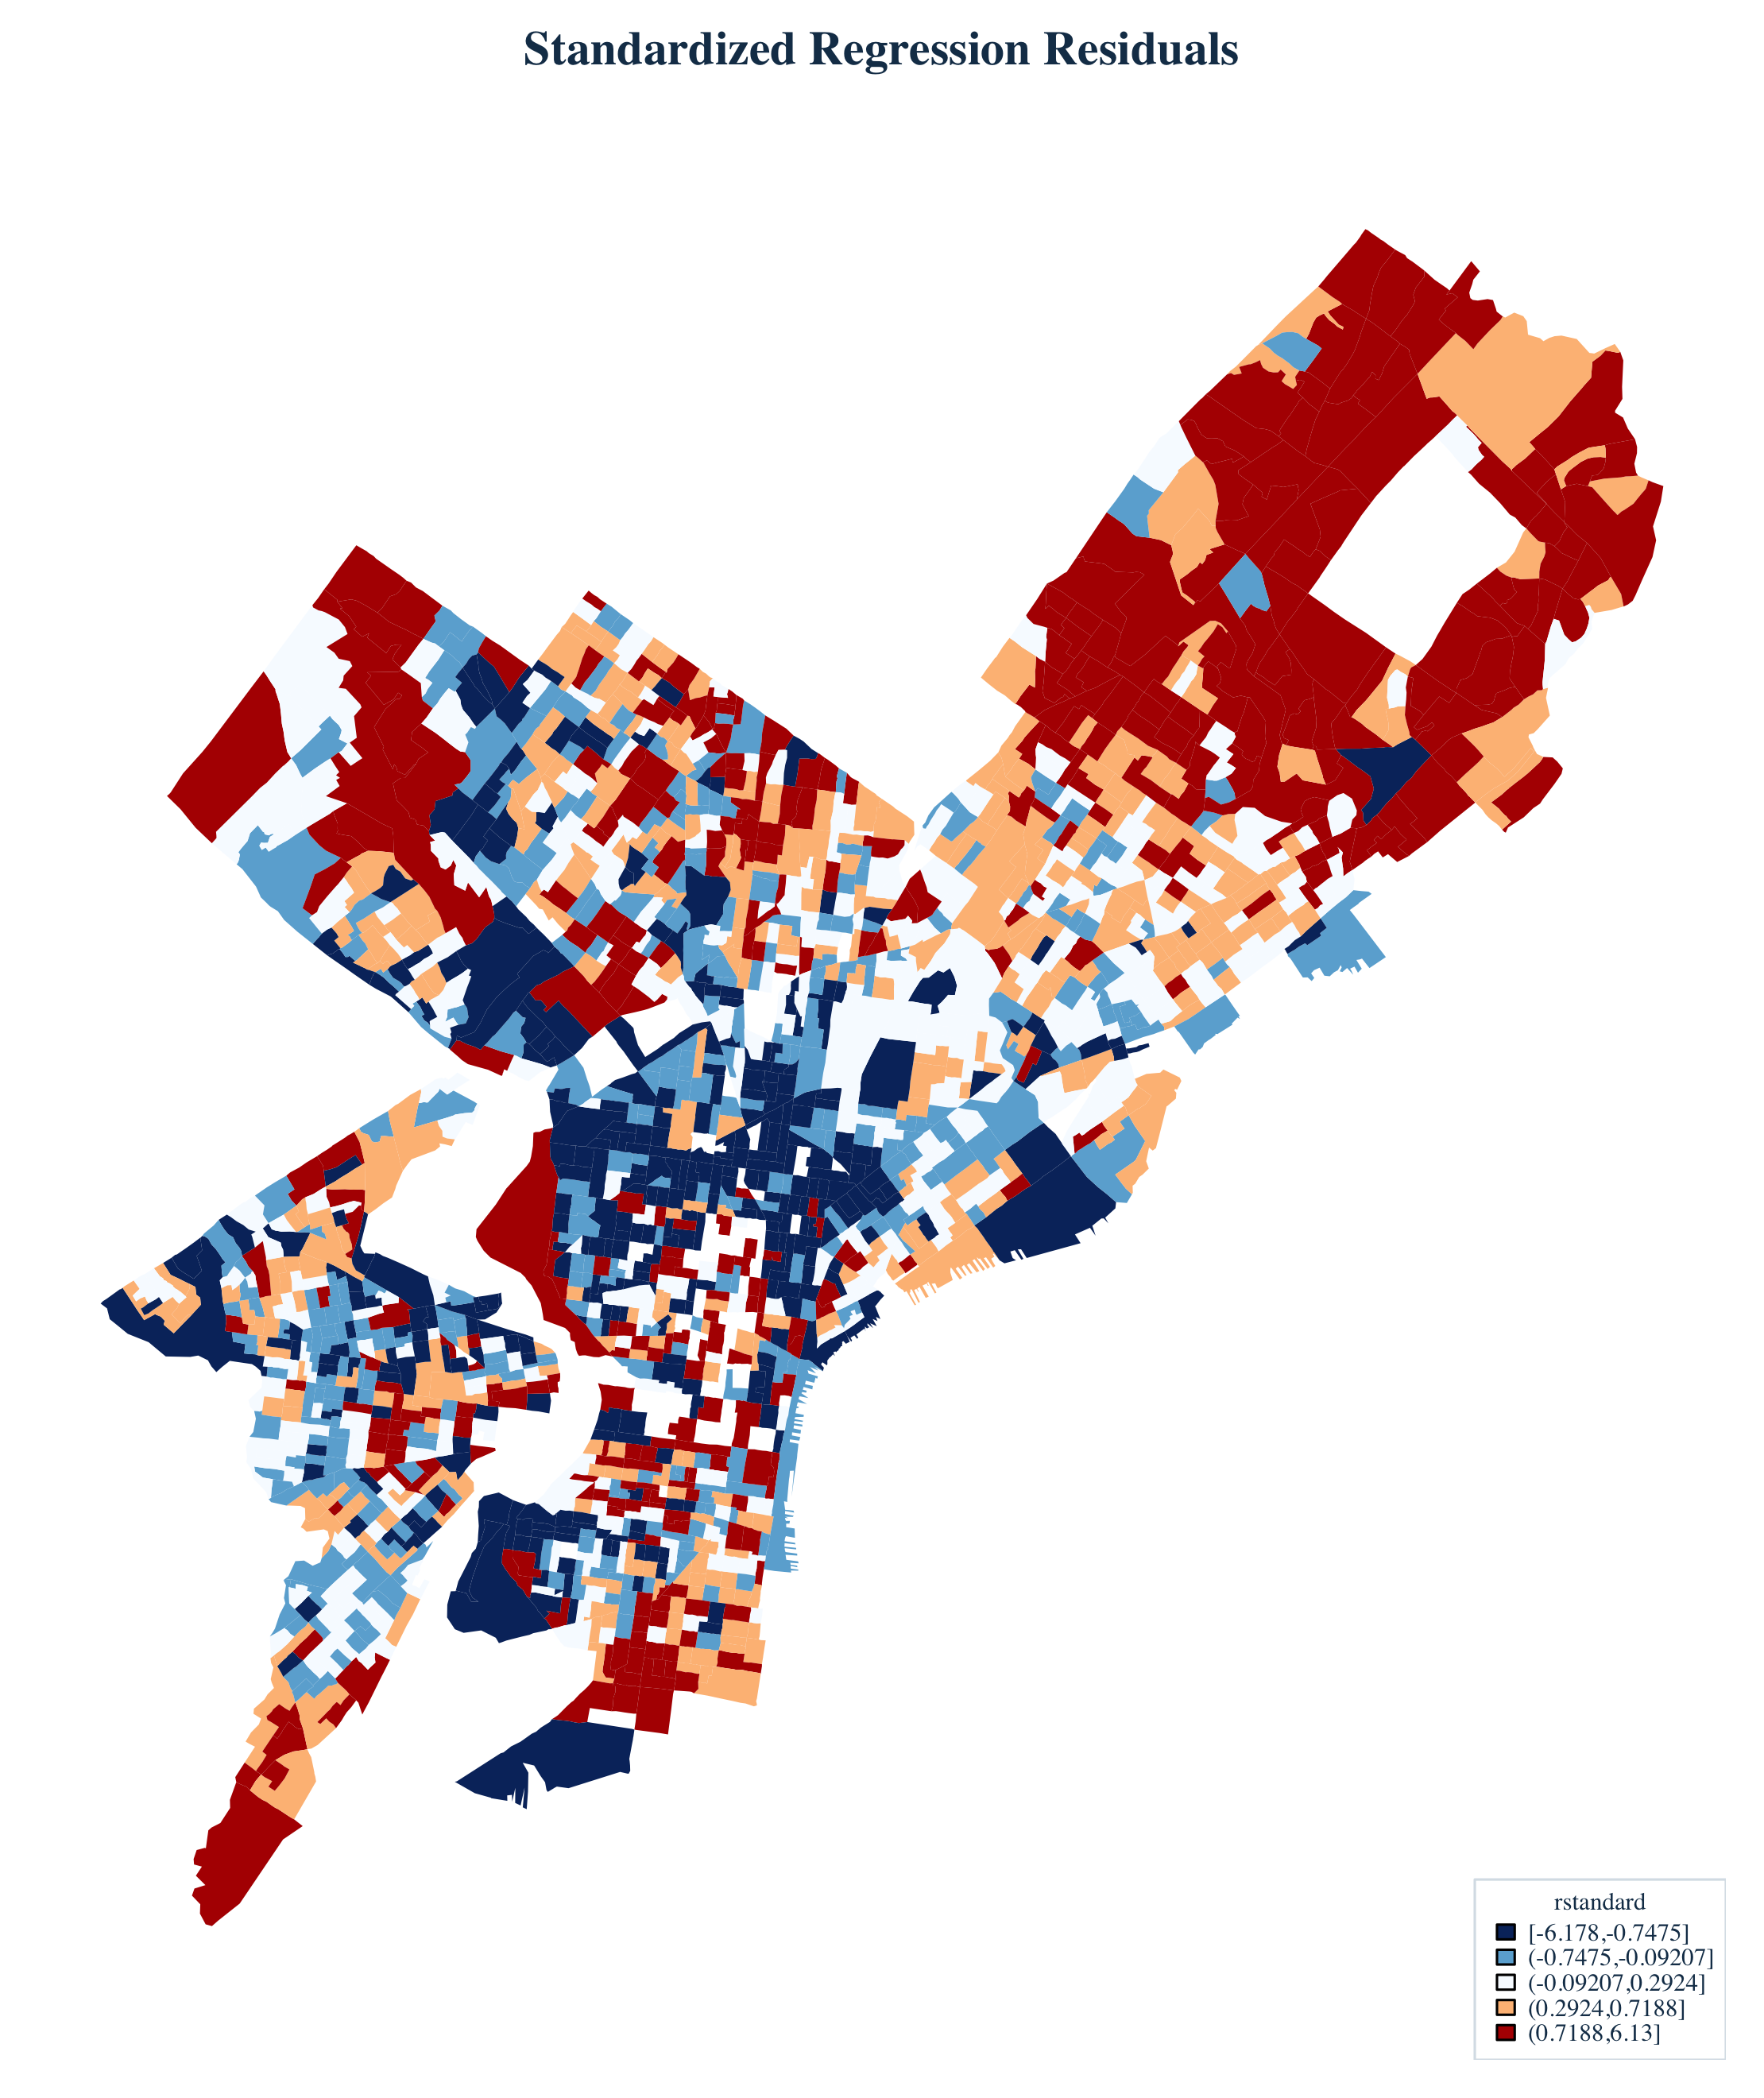
\includegraphics[width=0.67\textwidth,height=0.79\textheight,keepaspectratio]{fig_07_residual_map.png}
\caption{Standardized regression residuals by block group.}
\label{fig:residual-map}
\end{figure}

\clearpage
\subsection{Additional Models}

Do we even need all four predictors? Removing any one of them raised the \var{step}/\var{extractAIC} score (Table~\ref{tab:stepwise}), and since lower is better, none of the simpler models won on the fit-complexity trade-off. These scores differ from \var{AIC(fit)} by an additive constant but give the same within-set ranking.

\begin{table}[H]
\centering
\caption{Stepwise comparison on the \var{extractAIC} scale}
\label{tab:stepwise}
\begin{tabular}{lrr}
\toprule
Model considered & Residual SS & AIC score \\
\midrule
Full four-predictor model & 230.34 & $-3448.1$ \\
Remove \var{PCTSINGLES} & 232.75 & $-3432.2$ \\
Remove \var{LNNBELPOV100} & 242.04 & $-3364.9$ \\
Remove \var{PCTVACANT} & 281.89 & $-3102.7$ \\
Remove \var{PCTBACHMOR} & 429.36 & $-2379.0$ \\
\bottomrule
\end{tabular}
\end{table}

Cross-validation judges by held-out prediction instead of in-sample fit. The four-predictor model had lower five-fold RMSE than the two-predictor alternative (Table~\ref{tab:cv}), a reduction of approximately 17.2\% using the exact unrounded values. Thus, within the two prespecified candidates and the same fold allocation, retaining the four predictors produced the smaller typical prediction error. These model comparisons support the original specification within the limited candidate set, while the diagnostic evidence continues to qualify its inferential interpretation.

\begin{table}[H]
\centering
\caption{Five-fold cross-validation results}
\label{tab:cv}
\begin{tabularx}{\textwidth}{lXr}
\toprule
Model & Predictors & RMSE \\
\midrule
Original model & \var{PCTVACANT}, \var{PCTSINGLES}, \var{PCTBACHMOR}, \var{LNNBELPOV100} & 0.367 \\
Two-predictor model & \var{PCTVACANT}, \var{MEDHHINC} & 0.444 \\
\bottomrule
\end{tabularx}
\end{table}

\section{Discussion and Limitations}

In short, all four predictors had the expected signs and were statistically significant: vacancy and poverty were associated with lower house values, whereas education and detached housing were associated with higher values. The model explained 66.2\% of log-value variation, leaving about one-third unexplained. These estimates describe conditional associations in the observed block groups and should not be interpreted as causal effects.

Stepwise selection and cross-validation support the four-predictor specification within the candidate set, but they do not establish causality or a correct functional form. Crime, school quality, access, housing condition, taxes, and amenities remain plausible omitted variables. If these omitted factors are related to both the included predictors and house values, the estimated coefficients may partly reflect their influence.

The diagnostic evidence identifies additional reasons for caution. Curvature, heavy tails, heteroscedasticity, and spatial clustering weaken conventional OLS inference because they challenge the functional-form, distributional, variance, and independence assumptions. Robust standard errors, nonlinear terms, Moran's I, and spatial regression would improve the model. Random folds may also understate error when nearby block groups enter both training and test sets; spatially blocked validation is preferable.

The measurement of poverty creates a further limitation that is distinct from the regression diagnostics. \var{NBELPOV100} is a raw count, so it mixes poverty concentration with block-group size. Logging reduces skew but does not supply the missing denominator; a poverty rate plus total households would be clearer and would separate neighborhood poverty prevalence from the number of households at risk.

Finally, regularization offers a useful contrast with the selection approach used here. Ridge and LASSO shrink coefficients to reduce variance and overfitting. Ridge uses an L2 penalty and usually retains all variables, whereas LASSO uses an L1 penalty and can set coefficients to zero. With four predictors and a maximum pairwise correlation of 0.32, regularization is unnecessary here but may help in a larger model. Overall, the current regression is informative as a concise description of conditional housing-value patterns, but its diagnostic and measurement limitations should guide any subsequent extension.

\par\vspace{0.55em}
{\large\bfseries\color{navy}Reference\par}
\vspace{0.15em}
Rosen, S. (1974). Hedonic prices and implicit markets: Product differentiation in pure competition. \textbf{Journal of Political Economy, 82}(1), 34--55. \url{https://doi.org/10.1086/260169}

\end{document}
